\documentclass{standalone}
\usepackage{tikz}
\usetikzlibrary{patterns, positioning}
\usetikzlibrary{shapes.misc}
\usepackage[outline]{contour}
\contourlength{1.5pt} 
\usepackage[sfdefault]{ClearSans} %% option 'sfdefault' activates Clear Sans as the default text font
\usepackage[T1]{fontenc}

\begin{document}
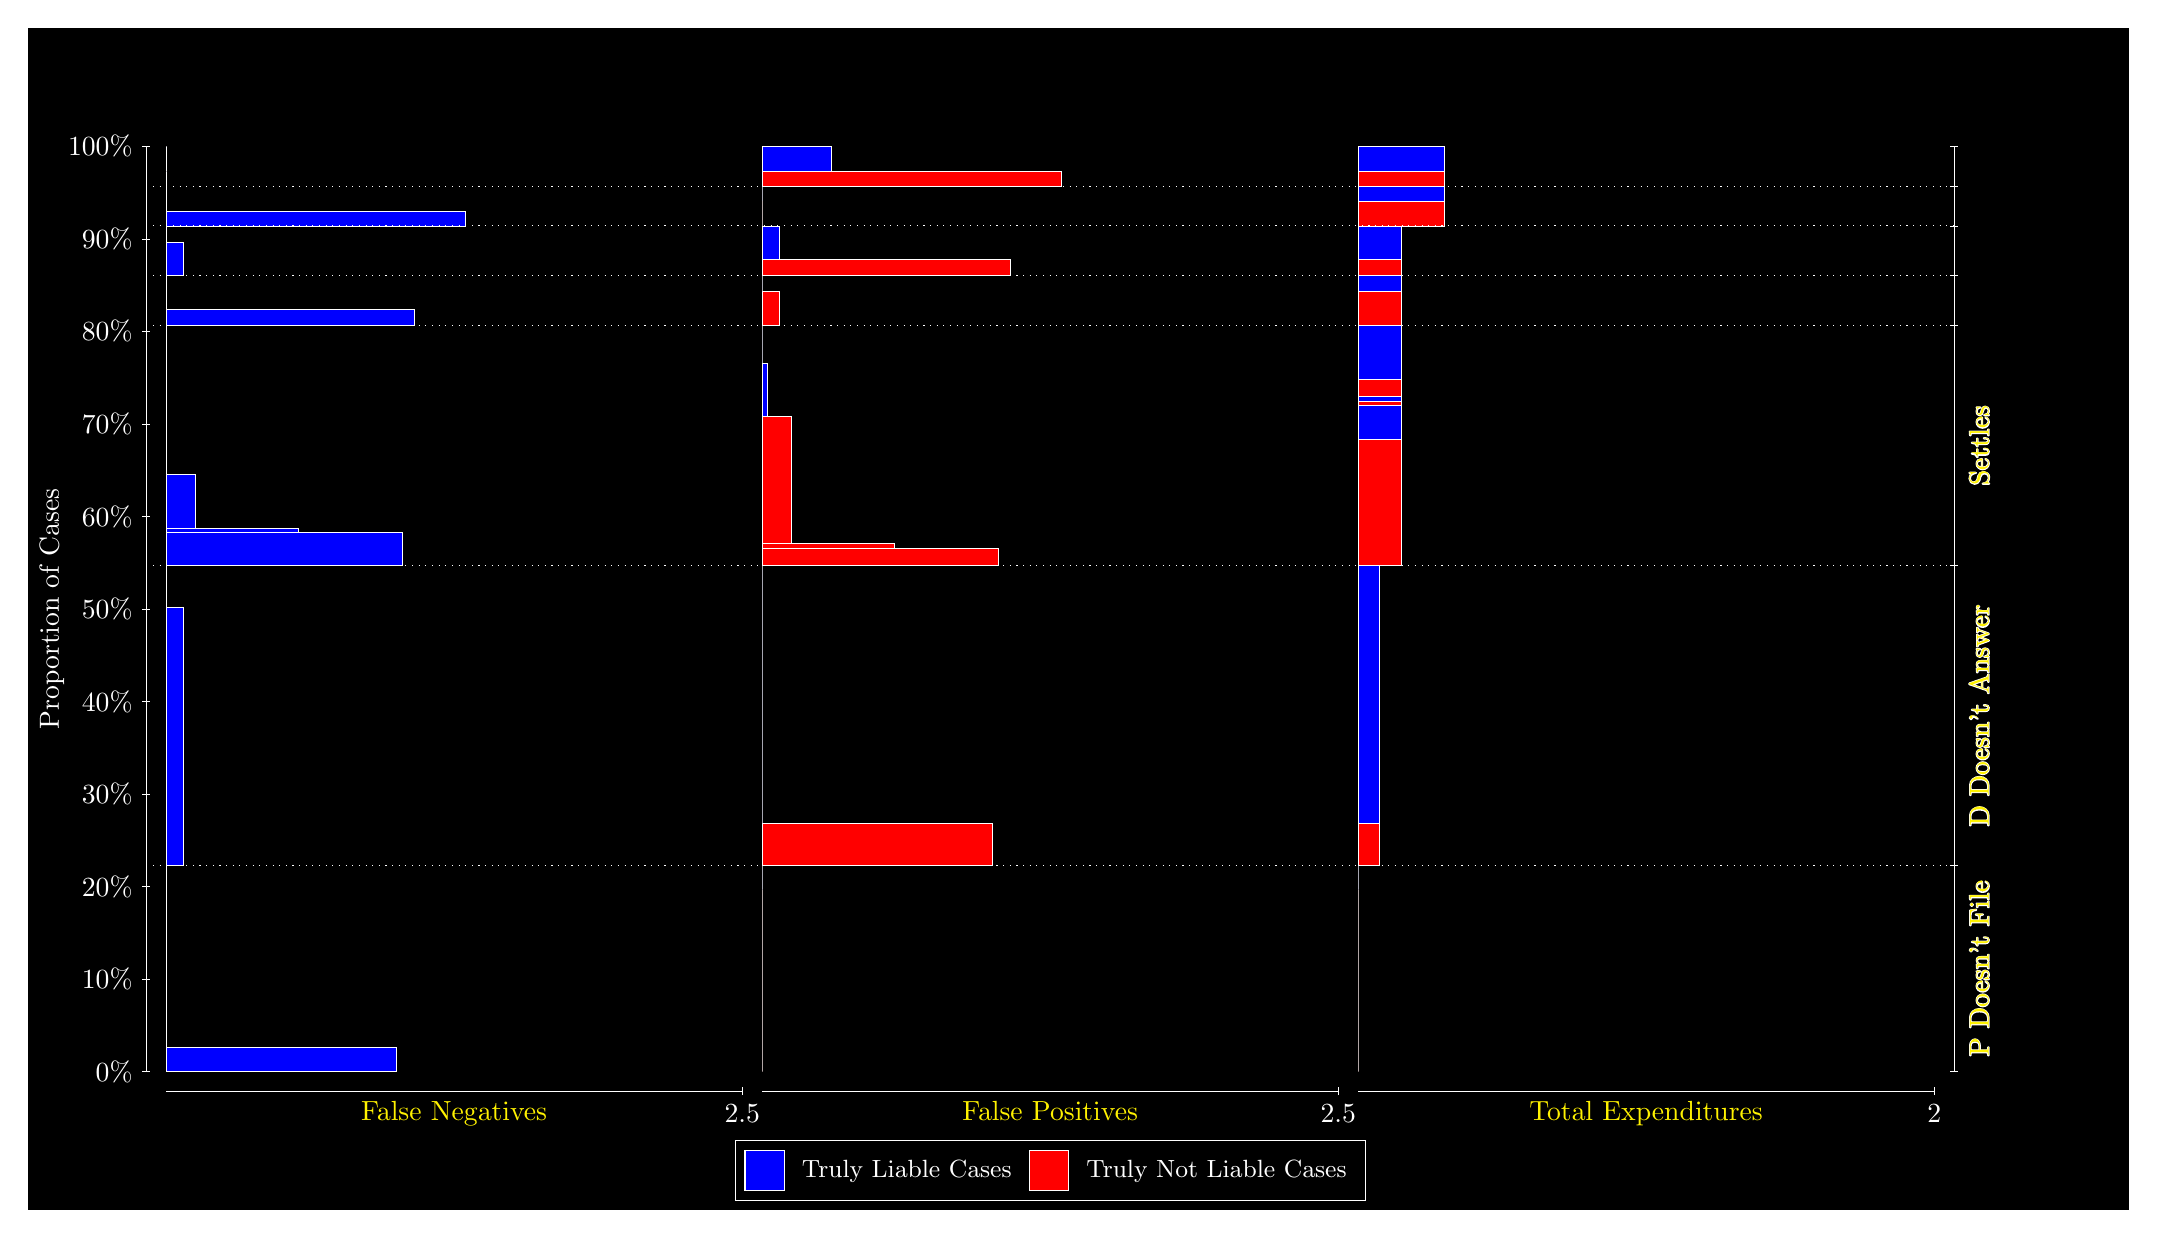
\begin{tikzpicture}
\draw[fill=black] (0,0) rectangle (26.667,15);
\draw[white, very thin] (1.5,1.75) -- (1.5,13.5);
\node[rotate=90, text=white, anchor=center] at (0.3, 7.625) {Proportion of Cases};
\draw[white, very thin] (1.45,1.75) -- (1.55,1.75);
\node[text=white, anchor=east] at (1.45, 1.75) {0\%};
\draw[white, very thin] (1.45,2.925) -- (1.55,2.925);
\node[text=white, anchor=east] at (1.45, 2.925) {10\%};
\draw[white, very thin] (1.45,4.1) -- (1.55,4.1);
\node[text=white, anchor=east] at (1.45, 4.1) {20\%};
\draw[white, very thin] (1.45,5.275) -- (1.55,5.275);
\node[text=white, anchor=east] at (1.45, 5.275) {30\%};
\draw[white, very thin] (1.45,6.45) -- (1.55,6.45);
\node[text=white, anchor=east] at (1.45, 6.45) {40\%};
\draw[white, very thin] (1.45,7.625) -- (1.55,7.625);
\node[text=white, anchor=east] at (1.45, 7.625) {50\%};
\draw[white, very thin] (1.45,8.8) -- (1.55,8.8);
\node[text=white, anchor=east] at (1.45, 8.8) {60\%};
\draw[white, very thin] (1.45,9.975) -- (1.55,9.975);
\node[text=white, anchor=east] at (1.45, 9.975) {70\%};
\draw[white, very thin] (1.45,11.15) -- (1.55,11.15);
\node[text=white, anchor=east] at (1.45, 11.15) {80\%};
\draw[white, very thin] (1.45,12.325) -- (1.55,12.325);
\node[text=white, anchor=east] at (1.45, 12.325) {90\%};
\draw[white, very thin] (1.45,13.5) -- (1.55,13.5);
\node[text=white, anchor=east] at (1.45, 13.5) {100\%};

\draw[white, very thin] (24.457,1.75) -- (24.457,13.5);
\draw[white, very thin] (24.407,1.75) -- (24.507,1.75);
\node[anchor=west] at (24.407, 1.75) {};
\draw[white, very thin] (24.407,4.366) -- (24.507,4.366);
\node[anchor=west] at (24.407, 4.366) {};
\draw[white, very thin] (24.407,8.173) -- (24.507,8.173);
\node[anchor=west] at (24.407, 8.173) {};
\draw[white, very thin] (24.407,11.226) -- (24.507,11.226);
\node[anchor=west] at (24.407, 11.226) {};
\draw[white, very thin] (24.407,11.858) -- (24.507,11.858);
\node[anchor=west] at (24.407, 11.858) {};
\draw[white, very thin] (24.407,12.489) -- (24.507,12.489);
\node[anchor=west] at (24.407, 12.489) {};
\draw[white, very thin] (24.407,12.994) -- (24.507,12.994);
\node[anchor=west] at (24.407, 12.994) {};
\draw[white, very thin] (24.407,13.5) -- (24.507,13.5);
\node[anchor=west] at (24.407, 13.5) {};

\draw[white, very thin, fill=blue] (1.75,1.75) rectangle (4.6775,2.0558);
\draw[white, very thin, fill=red] (1.75,2.0558) rectangle (1.75,4.366);
\draw[white, very thin, fill=blue] (1.75,4.366) rectangle (1.9696,7.6417);
\draw[white, very thin, fill=red] (1.75,7.6417) rectangle (1.75,8.173);
\draw[white, very thin, fill=blue] (1.75,8.173) rectangle (4.7507,8.5931);
\draw[white, very thin, fill=blue] (1.75,8.5931) rectangle (3.4333,8.6489);
\draw[white, very thin, fill=blue] (1.75,8.6489) rectangle (2.1159,9.3299);
\draw[white, very thin, fill=red] (1.75,9.3299) rectangle (1.75,11.226);
\draw[white, very thin, fill=blue] (1.75,11.226) rectangle (4.8971,11.429);
\draw[white, very thin, fill=red] (1.75,11.429) rectangle (1.75,11.858);
\draw[white, very thin, fill=blue] (1.75,11.858) rectangle (1.9696,12.286);
\draw[white, very thin, fill=red] (1.75,12.286) rectangle (1.75,12.489);
\draw[white, very thin, fill=blue] (1.75,12.489) rectangle (5.5558,12.676);
\draw[white, very thin, fill=red] (1.75,12.676) rectangle (1.75,12.994);
\draw[white, very thin, fill=red] (1.75,12.994) rectangle (1.75,13.182);
\draw[white, very thin, fill=blue] (1.75,13.182) rectangle (1.75,13.5);
\draw[white, very thin, fill=red] (9.3189,1.75) rectangle (9.3189,4.0603);
\draw[white, very thin, fill=blue] (9.3189,4.0603) rectangle (9.3189,4.366);
\draw[white, very thin, fill=red] (9.3189,4.366) rectangle (12.246,4.8974);
\draw[white, very thin, fill=blue] (9.3189,4.8974) rectangle (9.3189,8.173);
\draw[white, very thin, fill=red] (9.3189,8.173) rectangle (12.32,8.3952);
\draw[white, very thin, fill=red] (9.3189,8.3952) rectangle (11.002,8.4578);
\draw[white, very thin, fill=red] (9.3189,8.4578) rectangle (9.6848,10.07);
\draw[white, very thin, fill=blue] (9.3189,10.07) rectangle (9.3921,10.751);
\draw[white, very thin, fill=blue] (9.3189,10.751) rectangle (9.3189,11.226);
\draw[white, very thin, fill=red] (9.3189,11.226) rectangle (9.5384,11.655);
\draw[white, very thin, fill=blue] (9.3189,11.655) rectangle (9.3189,11.858);
\draw[white, very thin, fill=red] (9.3189,11.858) rectangle (12.466,12.06);
\draw[white, very thin, fill=blue] (9.3189,12.06) rectangle (9.5384,12.489);
\draw[white, very thin, fill=red] (9.3189,12.489) rectangle (9.3189,12.806);
\draw[white, very thin, fill=blue] (9.3189,12.806) rectangle (9.3189,12.994);
\draw[white, very thin, fill=red] (9.3189,12.994) rectangle (13.125,13.182);
\draw[white, very thin, fill=blue] (9.3189,13.182) rectangle (10.197,13.5);
\draw[white, very thin, fill=red] (16.888,1.75) rectangle (16.888,4.0603);
\draw[white, very thin, fill=blue] (16.888,4.0603) rectangle (16.888,4.366);
\draw[white, very thin, fill=red] (16.888,4.366) rectangle (17.162,4.8974);
\draw[white, very thin, fill=blue] (16.888,4.8974) rectangle (17.162,8.173);
\draw[white, very thin, fill=red] (16.888,8.173) rectangle (17.437,9.7849);
\draw[white, very thin, fill=blue] (16.888,9.7849) rectangle (17.437,10.205);
\draw[white, very thin, fill=red] (16.888,10.205) rectangle (17.437,10.268);
\draw[white, very thin, fill=blue] (16.888,10.268) rectangle (17.437,10.323);
\draw[white, very thin, fill=red] (16.888,10.323) rectangle (17.437,10.546);
\draw[white, very thin, fill=blue] (16.888,10.546) rectangle (17.437,11.226);
\draw[white, very thin, fill=red] (16.888,11.226) rectangle (17.437,11.655);
\draw[white, very thin, fill=blue] (16.888,11.655) rectangle (17.437,11.858);
\draw[white, very thin, fill=red] (16.888,11.858) rectangle (17.437,12.06);
\draw[white, very thin, fill=blue] (16.888,12.06) rectangle (17.437,12.489);
\draw[white, very thin, fill=red] (16.888,12.489) rectangle (17.986,12.806);
\draw[white, very thin, fill=blue] (16.888,12.806) rectangle (17.986,12.994);
\draw[white, very thin, fill=red] (16.888,12.994) rectangle (17.986,13.182);
\draw[white, very thin, fill=blue] (16.888,13.182) rectangle (17.986,13.5);
\draw[white, dotted] (1.5,4.366) -- (24.457,4.366);
\draw[white, dotted] (1.5,8.173) -- (24.457,8.173);
\draw[white, dotted] (1.5,11.226) -- (24.457,11.226);
\draw[white, dotted] (1.5,11.858) -- (24.457,11.858);
\draw[white, dotted] (1.5,12.489) -- (24.457,12.489);
\draw[white, dotted] (1.5,12.994) -- (24.457,12.994);
\draw[white, very thin] (1.75,1.5) -- (9.0689,1.5);
\node[text=yellow, anchor=north] at (5.4094, 1.5) {False Negatives};
\draw[white, very thin] (9.0689,1.45) -- (9.0689,1.55);
\node[text=white, anchor=north] at (9.0689, 1.45) {2.5};

\draw[white, very thin] (9.3189,1.5) -- (16.638,1.5);
\node[text=yellow, anchor=north] at (12.978, 1.5) {False Positives};
\draw[white, very thin] (16.638,1.45) -- (16.638,1.55);
\node[text=white, anchor=north] at (16.638, 1.45) {2.5};

\draw[white, very thin] (16.888,1.5) -- (24.207,1.5);
\node[text=yellow, anchor=north] at (20.547, 1.5) {Total Expenditures};
\draw[white, very thin] (24.207,1.45) -- (24.207,1.55);
\node[text=white, anchor=north] at (24.207, 1.45) {2};

\node[text=yellow, centered, rotate=90] at (24.777, 3.058) {\contour{white}{P Doesn't File}};
\node[text=yellow, centered, rotate=90] at (24.777, 6.2695) {\contour{white}{D Doesn't Answer}};
\node[text=yellow, centered, rotate=90] at (24.777, 9.6998) {\contour{white}{Settles}};





\draw (12.978300999999998,1.5) node[draw=none] (baseCoordinate) {};
\begin{scope}[align=center]
        \matrix[scale=0.5, draw=white, below=0.5cm of baseCoordinate, nodes={draw}, column sep=0.1cm]{
            \node[rectangle, draw, minimum width=0.5cm, minimum height=0.5cm, fill=blue] {}; &
            \node[draw=none, font=\small, text=white] (B) {Truly Liable Cases}; &
            \node[rectangle, draw, minimum width=0.5cm, minimum height=0.5cm, fill=red] {}; &
            \node[draw=none, font=\small, text=white] (B) {Truly Not Liable Cases}; \\
            };
\end{scope}

\end{tikzpicture}
\end{document}